\section{Bayesian Calibration}
\label{sec:bayes}

As discussed earlier in Section~\ref{sec:intro}, the underlying methodology for determining the nominal 
estimates for SW potential parameters did not account for measurement error, inadequate functional
form of the potential, inherent noise in MD predictions, and parametric uncertainties. Hence, there is
a possibility of improving the estimates since using the same set of values for a wide variety of systems
and applications is not ideal. A robust approach to calibrating the parameters in the presence of
such uncertainties is made possible by using a Bayesian framework. The methodology aims at evaluating
the so-called joint posterior probability distribution (referred to as the `posterior') of the uncertain model 
parameters to be calibrated, using Bayes' rule:

\be
\mathcal{P}(\bm{X}\vert \bm{Y}) \propto \mathcal{P}(\bm{Y}\vert\bm{X})\mathcal{P}(\bm{X})
\ee

\noindent where $\bm{X}$ is the set of uncertain model parameters, and $\bm{Y}$ is the available set of
experimental data i.e. bulk thermal conductivity at different temperatures in the present case. 
We exploit our findings based on sensitivity analysis in
Figure~\ref{fig:gsa} and focus on calibrating $\alpha$ and $\gamma$ i.e. $\bm{X}:\{\alpha,\gamma\}$.
$\mathcal{P}(\bm{X}\vert \bm{Y})$ is regarded as the posterior, $\mathcal{P}(\bm{Y}\vert\bm{X})$ is the
`likelihood', and $\mathcal{P}(\bm{X})$ is the joint prior probability distribution (referred to as the `prior') of $\bm{X}$.
The likelihood accounts for measurement error, and the discrepancy between experiments and model
predictions, whereas, the prior is an initial guess for the distribution of uncertain model parameters in an
interval. It also accounts for the availability of the expert opinion pertaining to their estimates. 
The posterior provides an estimate of the most likely value of the uncertain model parameters based on
prior uncertainty, experimental data used for calibration and the associated measurement error, and model
discrepancy. Additionally, the posterior is often used to quantify the uncertainty associated with model predictions. Several algorithms based on the Markov chain Monte Carlo (MCMC) technique are available for  
sampling the posterior~\cite{Haario:2001, Haario:2006,Xu:2014}.

Evaluating the joint posterior of $\alpha$ and $\gamma$ using MCMC typically requires a large amount of
computational effort and is not the focus of this work. Instead, we compute and plot the joint likelihood on
a 2D cartesian grid described by $\alpha$ and $\gamma$ using Eq.~\ref{eq:like} as illustrated in
Figure~\ref{fig:like}(a). For this purpose, we consider the priors of $\alpha$ and $\gamma$ to be
independent and uniformly distributed in the intervals, [1.62,1.98] and [1.08,1.32] respectively. 
Consequently, the posterior is proportional to the likelihood, considered to be a Gaussian:

\be
\mathcal{P}(\bm{Y}\vert\bm{X}) = \frac{1}{\sqrt{2\pi\sigma^2}}\exp\left[-\frac{(\kappa_{\tiny{\mbox{E}}} - 
\kappa_{\tiny{\mbox{MD}}})^2}{2\sigma^2}\right]
\label{eq:like}
\ee

\noindent where $\sigma$ is the standard deviation of the measurement error, and
$(\kappa_{\tiny{\mbox{E}}} - \kappa_{\tiny{\mbox{MD}}})$ is the discrepancy between 
NEMD predictions~($\kappa_{\tiny{\mbox{MD}}}$)
and experimental data~($\kappa_{\tiny{\mbox{E}}}$). Experimental data for $\kappa_{\tiny{\mbox{E}}}$ at 300~K
(149~W/m/K~\cite{Shanks:1963}) is used to compute the joint likelihood. It must be noted that the likelihood
function in Eq.~\ref{eq:like} could be refined further by accounting for a model discrepancy term and hence
calibrating the associated parameters in addition to the uncertain model inputs~\cite{Kennedy:2001,Ling:2014}. 

\begin{figure}[htbp]
 \begin{center}
  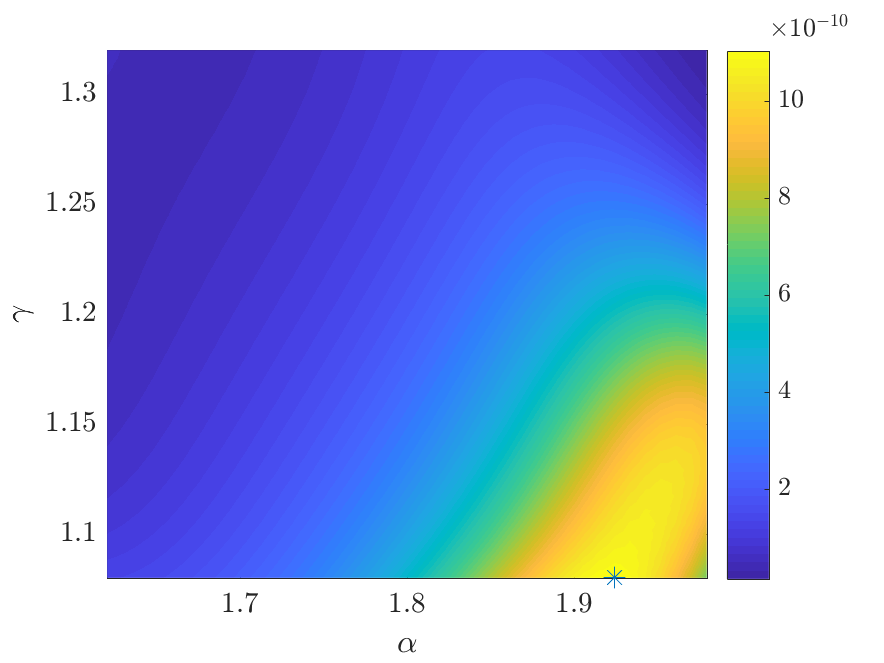
\includegraphics[width=0.70\textwidth]{./Figures/gl}
  \\ (a)
  \begin{tabular}{cc}
  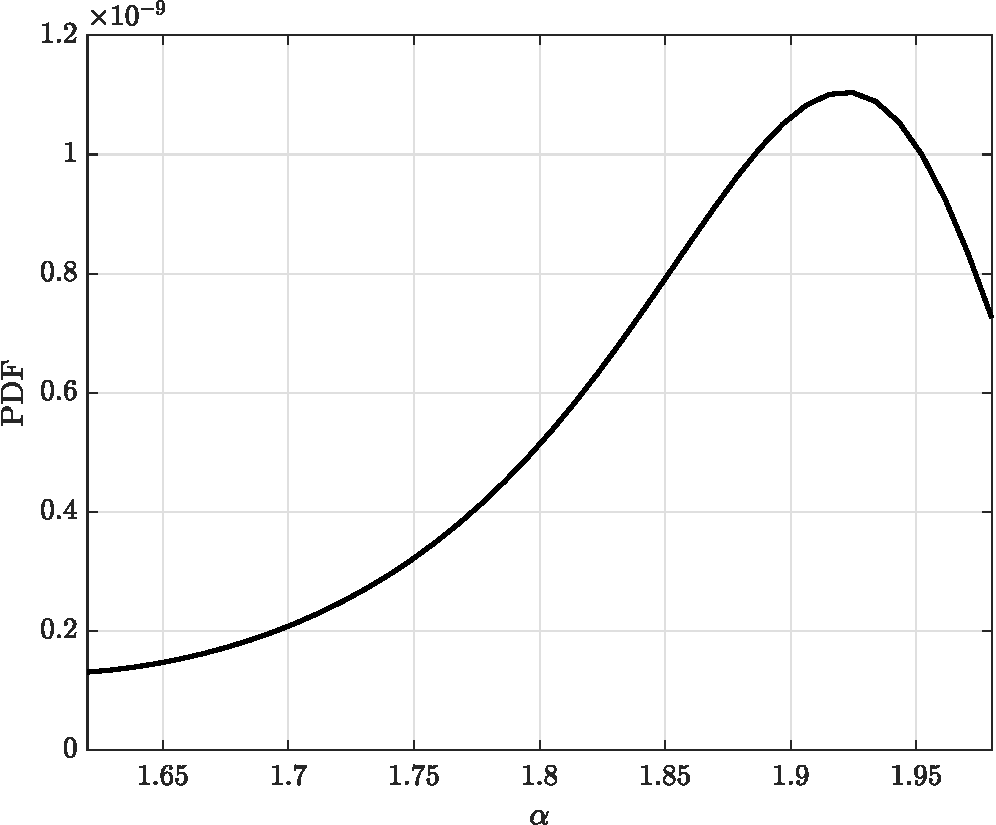
\includegraphics[width=0.50\textwidth]{./Figures/pdf_alpha}
  &
  %\hspace{3mm}
  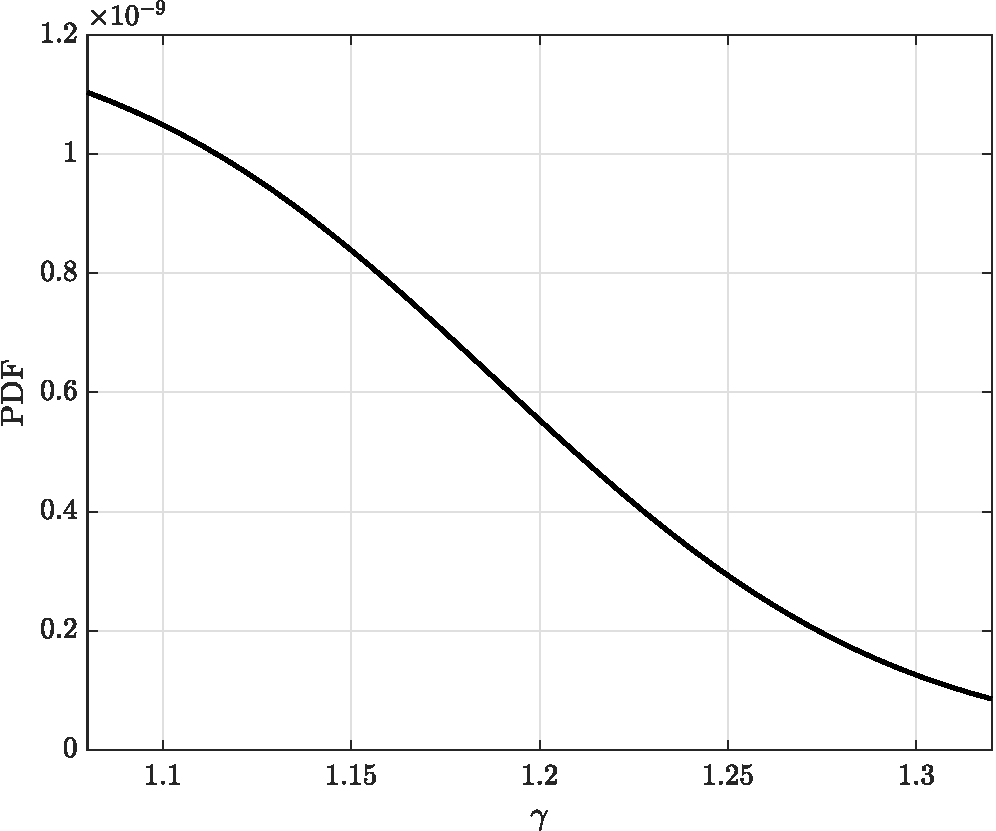
\includegraphics[width=0.50\textwidth]{./Figures/pdf_gamma}
  \\ (b) & (c)
  \end{tabular}
\caption{(a) The joint likelihood of ($\alpha$,$\gamma$) as estimated using Eq.~\ref{eq:like} is plotted
on a 2D cartesian grid. The maximum likelihood estimate (MLE) is also highlighted.
Marginal likelihoods for $\alpha$ and $\gamma$ are plotted in (b) and (c) respectively.}
\label{fig:like}
\end{center}
\end{figure}

Marginal distributions for
$\alpha$ and $\gamma$ are shown in Figure~\ref{fig:like}(b) and Figure~\ref{fig:like}(c) respectively. 
As mentioned above, the joint likelihood plot is based on the bulk thermal conductivity measurement at 300~K.
An enhanced set of experimental measurements at different bulk temperatures would help improve the
accuracy of the calibration process considering the measurement noise is not too large. Moreover, it would
help capture the correlation between calibration parameters across temperatures at which the data is
available. However, a reduced-order surrogate would be needed at each temperature in order to make the
MCMC tractable.  





















